\documentclass[en]{../../../eplsummary}

\usepackage{siunitx}
\usepackage{circuitikz}

\newcommand*\mean[1]{\overline{#1}}
\newcommand*\equal{=} % hack to have = in tikz

\hypertitle{Analog Electronics}{8}{ELEC}{2532}
{Antoine Paris}
{Denis Flandre}

\section{Electronic noise}
The reference for this section is~\cite[chapter~11]{gray}.
This section assumes the reader is familiar with concepts of variance,
covariance, stationarity, power spectral density, Wiener-Kintchine
theorem, etc. Nevertheless, a very brief summary will be given in the
first section. Please refer to the stochastic processes course otherwise.

\subsection{Notations and reminders}
Let $x(t)$ be a noisy (i.e. random) signal (a voltage or a current in this case).
The notation $\mean{x^2}$ corresponds to the mean-square variation of $x$
around its average value $\mu_x$
\begin{align*}
    \mean{x^2}  &= \mean{(x-\mu_x)^2} \\
                &= \lim_{T\to\infty}\frac{1}{T}\int_0^T (x-\mu_x)^2
                \mathrm{d}t.
\end{align*}
In other words, $\mean{x^2}$ is the variance of $x$, $\sigma^2_x$.
In this course, we will often write this as
\begin{equation}
    \mean{x^2} = S(f)\Delta f
    \label{eq:var-psd}
\end{equation}
where $S(f)$ is the power spectral density and $\Delta f$ is the bandwidth
of interest. From the stochastic processes course, you may remember that
the variance can more rigorously be obtained by
\begin{equation}
    \sigma^2 = \int_{-F}^F S(f) \mathrm{d}f
    \label{eq:psd}
\end{equation}
where $S(f)$ is again the power spectral density and the bandwidth of
interest $\Delta f = 2F$. Intuitively, we see that $S(f)$ (expressed either
in either \SI{}{\volt\squared\per\hertz} or \SI{}{\ampere\per\hertz}) gives
how energy is distributed in the frequency domain.
From equation~\eqref{eq:psd}, we can see that equation~\eqref{eq:var-psd}
is only valid if
\begin{enumerate}
    \item $S(f)$ is constant w.r.t the frequency. In this case, $x$ is said to be
    a \emph{white noise} and equation~\eqref{eq:var-psd} is exact. As a reminder,
    the power spectral density is defined as
    the Fourier transform of the auto-covariance function of a weak-sense stationary
    random process. A constant power spectral density thus means that the
    auto-covariance function is a delta, i.e. that the given random process at different
    time instants is uncorrelated ;
    \item The bandwidth of interest $\Delta f$ is small, so that $S(f)$ can be
    considered to be constant on this limited bandwidth. In this case,
    equation~\eqref{eq:var-psd} is only an approximation.
\end{enumerate}
Finally, the corresponding root-mean-square (a.k.a. rms) value is simply given
by
\[ x = \sqrt{\mean{x^2}} = \sqrt{S(f)\Delta f}. \]
Figure~\ref{fig:noise-eq-sin} illustrates equation~\eqref{eq:var-psd} in the
case of a noise current. It also shows why we can approximate noise current
with power spectral density $S(f)$ on a bandwidth $\Delta f$ by a sinusoidal
current generator with rms value $i = \sqrt{\S(f)\Delta f}$.

\begin{figure}[ht]
    \centering
    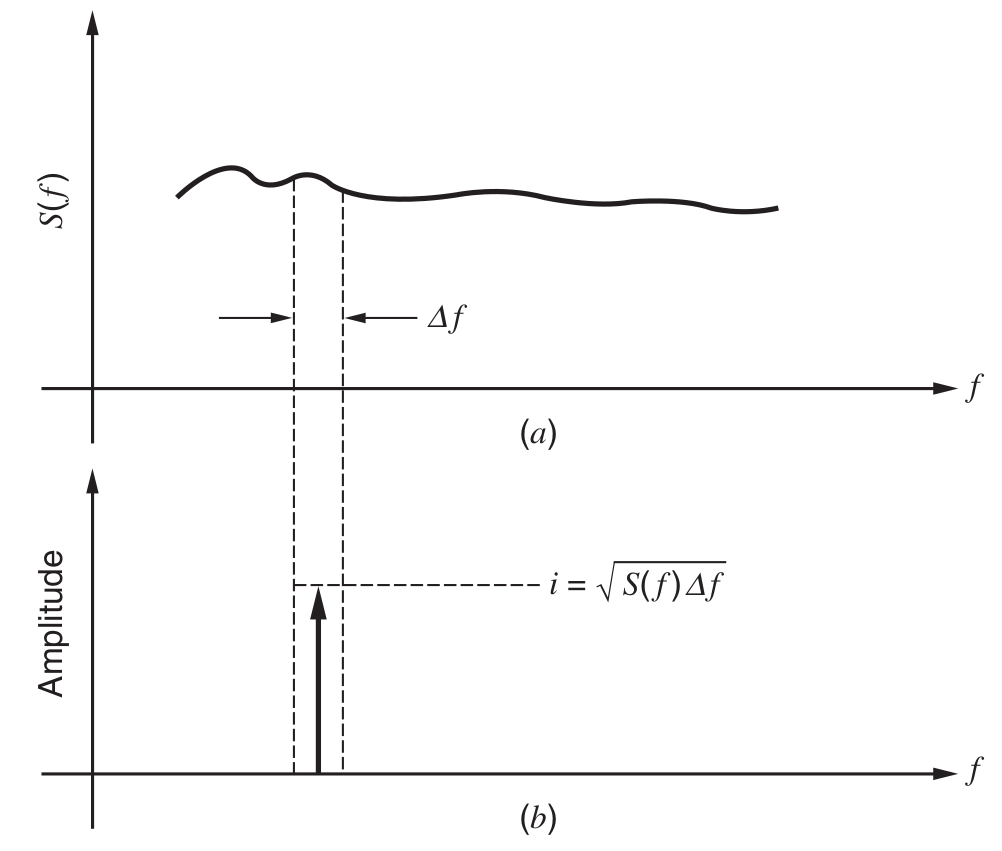
\includegraphics[width=0.5\textwidth]{figures/noise-eq-sin.png}
    \caption{Representation of noise in a bandwidth $\Delta f$ by an
    equivalent sinusoid with the same rms value.}
    \label{fig:noise-eq-sin}
\end{figure}

\subsection{Sources of noise}
\subsubsection{Thermal noise}
In conventional resistors, it is due to the \emph{random thermal motion of
the electrons} and is unnafected by the presence or absence of direct
current. In a resistor $R$, thermal noise can be represented by a series
voltage generator of mean square value $\mean{v^2}$ or by a shunt current
generator of mean square value $\mean{i^2}$
\begin{align*}
    \mean{v^2} &= 4kTR\Delta f, \\
    \mean{i^2} &= 4kT\frac{1}{R}\Delta f,
\end{align*}
where $k$ is the Boltzmann's constant, $T$ the absolute temperature (i.e. in
Kelvin) and $\Delta f$ the bandwidth in Hertz. This is illustrated in figure
~\ref{fig:thermal-noise-repr}.
From this, it is clear that thermal noise is a \textbf{white noise}. Indeed,
its power spectral density is given either by $4kTR$ in \SI{}{\volt\squared
\per\hertz} or by $4kT\frac{1}{R}$ in \SI{}{\ampere\squared\per\hertz} and
is constant as a function of frequency (this is true up to \SI{1e13}{\hertz}).
Finally, the instantaneous amplitude distribution of thermal noise is
\textbf{Gaussian}.

\begin{figure}[ht]
    \centering
    \begin{circuitikz}
        \draw
        (0,0) to[short, o-] (0,-0.5)
        (0,-0.5) to[R, l=$R$] (0,-2)
        (0,-3.5) to[V, v=$\mean{v^2}$] (0,-2)
        (0,-3.5) to[short, -o] (0,-4)
        
        (5,0) to[short, o-*] (5,-0.5)
        (5,-0.5) to[R, l=$R$] (5,-3.5)
        (5,-3.5) to[short, *-o] (5,-4)
        (5,-0.5) -- (7,-0.5) to[I, i=$\mean{i^2}$] (7,-3.5) -- (5,-3.5)
        ;
    \end{circuitikz}
    \caption{Representations of thermal noise. The noise voltage (resp. current) is
    represented by a sinusoidal voltage (resp. current) generator with rms value
    $v$ (resp $i$). 
    Note that, because the only quantity of interest is the mean-square value,
    the polarity of the sources doesn't matter.}
    \label{fig:thermal-noise-repr}
\end{figure}

\subsubsection{Shot noise}
Shot noise is always associated with a direct-current flow and is present in
diodes, MOS transistors and bipolar transistors (i.e. devices for which
a potential barrier across a junction exists). The passage of each carrier
across the junction can be modeled as a random event (which depends on
carrier's energy, direction, etc). The external current is thus composed of
a large number of random independent current pulses. Noting $I_J$ the average
current across the junction, the noise current has a mean square given by
\[ \mean{i^2} = 2qI_J\Delta f \]
where $q$ is the electronic charge. As for thermal noise, this is a
\textbf{white noise} with a \textbf{Gaussian} amplitude distribution.
A small-signal model of a diode including the effect of shot noise is
illustrated in figure~\ref{fig:shot-noise-diode-repr}.
Finally, shot noise is non-correlated with thermal noise. Because shot noise
and thermal noise are both Gaussian, this means that they are independent.

%TODO: why polarity of the source doesn't matter
\begin{figure}[ht]
    \centering
    \begin{circuitikz}
        \draw
        (2,0) to[short, o-] (2,-0.5)
        (2,-0.5) to[D, i=$I_D$] (2,-2.5)
        (2,-2.5) to[short, -o] (2,-3)
        
        (5,0) -- (8,0) to[I, i=$\mean{i^2}\equal2qI_D\Delta f$] (8,-3)
        (8,-3) -- (5,-3) to[R, l=$r_d\equal\frac{kT}{qI_D}$] (5,0)
        ;
    \end{circuitikz}
    \caption{Diode small signal model including the effect of shot noise.
    Note that the small signal resistance $r_d$ of the diode is not an actual
    resistance (i.e. that's just a model of the diode). As such, it is not
    a source of thermal noise.}
    \label{fig:shot-noise-diode-repr}
\end{figure}

\subsubsection{Flicker noise}
Flicker noise (also called pink noise, or $1/f$ noise) is a type of noise
found in all active devices, as well as in some discrete passive elements
such as carbon resistors. The origins of flicker noise are varied, but it is
caused mainly by traps associated with contamination and crystal defects.
Flicker noise is always associated with a flow of direct current, the noise
current has a mean square given by
\[ \mean{i^2} = K_1\frac{I^a}{f^a}\Delta f \]
where $\Delta f$ is a small bandwidth around $f$\footnote{Indeed, remember
the discussion about equation~\ref{eq:var-psd}.}, $I$ is the direct current,
$K_1$, $a$ and $b \approx 1$ are technology parameters.
At the opposite of thermal noise and shot noise, flicker noise is \textbf{not
white} (hence the name pink) and often has a \textbf{non-Gaussian} amplitude
distribution.

%TODO: might be better in a table in fact...
\subsubsection{Summary}
A summary of the different noise sources is given in
figure~\ref{fig:noise-summary}.

\begin{figure}[ht]
    \centering
    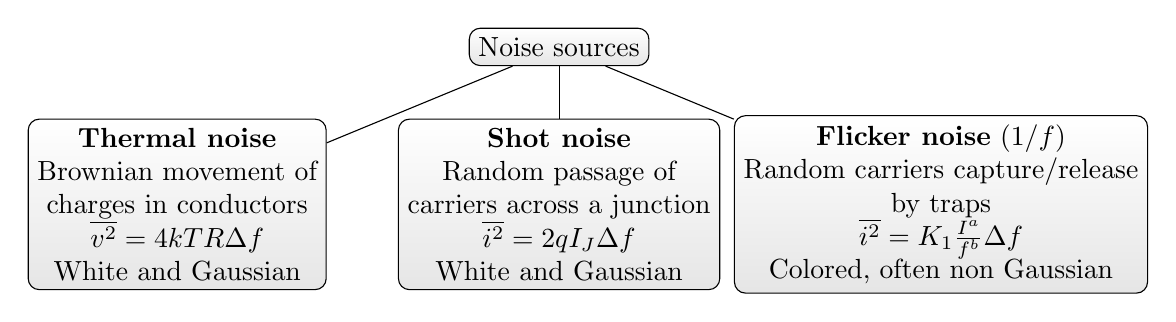
\begin{tikzpicture}[level distance=2cm,
        level 1/.style = {sibling distance = 0.4\textwidth},
        every node/.style = {shape=rectangle, rounded corners,
        draw, align=center,
        top color=white, bottom color=gray!20}]

        \node {Noise sources}
            child { node {\textbf{Thermal noise}\\
            Brownian movement of\\
            charges in conductors\\
            $\mean{v^2} = 4kTR\Delta f$\\
            White and Gaussian}  }
            child { node {\textbf{Shot noise}\\
            Random passage of\\
            carriers across a junction\\
            $\mean{i^2} = 2qI_J\Delta f$\\
            White and Gaussian} }
            child { node {\textbf{Flicker noise} ($1/f$)\\
            Random carriers capture/release\\
            by traps\\
            $\mean{i^2} = K_1\frac{I^a}{f^b}\Delta f$\\
            Colored, often non Gaussian} };    
    \end{tikzpicture}
    \caption{Summary of the different noise sources.}
    \label{fig:noise-summary}
\end{figure}

\subsection{Noise models of Integrated-Circuit Components}
\subsubsection{Resistors}
Monolithic and thin-film resistors display thermal noise. This has already
been illustrated in figure~\ref{fig:thermal-noise-repr}.

\subsubsection{Capacitors and inductors}
There are \emph{no sources of noise} in \emph{ideal} capacitors or
inductors. In practice, however, real components have parasitic resistances
that does display thermal noise.

\subsubsection{Junction Diode}
A small-signal model of the diode that includes the effect of shot noise was
already given in figure~\ref{fig:shot-noise-diode-repr}. This one, however,
does not take into account neither the series parasitic resistance of the
diode (which will display thermal noise) or flicker noise. A more complete
model is given in figure~\ref{fig:diode-noise-model}.

\begin{figure}[ht]
    \centering
    \begin{circuitikz}
        \draw 
        (1.5, 3.3) to[short, o-] (1.5, 3) 
        (1.5, 3) to[V, v=$\mean{v^2_s}\equal4kTr_s\Delta f$] (1.5, 1.5)
        (1.5, 1.5) to[R, l=$r_s$] (1.5, 0) to[short, -*] (1.5, 0)
        (0,0) -- (3,0) to[I, i=$\mean{i^2}\equal2qI_D\Delta f
        + K\frac{I_D^a}{f^b}\Delta f$] (3,-3)
        (3,-3) -- (0,-3) to[R, l=$r_d\equal\frac{kT}{qI_D}$] (0,0)
        (1.5, -3) to[short, -o] (1.5, -3.3)
        ;
    \end{circuitikz}
    \caption{Complete diode small-signal model equivalent circuit with noise
    sources.}
    \label{fig:diode-noise-model}
\end{figure}

\subsubsection{Bipolar transistor}
A small-signal model equivalent circuit with noise sources for a bipolar transistor
is given in figure~\ref{fig:bjt-noise-model}. This model contains the following
noise sources:
\begin{enumerate}
	\item $\mean{v^2_b}$: thermal noise associated with the
	parasitic resistance of the base connection
	\[ \mean{v^2_b} = 4kTr_b\Delta f. \]
	\item $\mean{i^2_c}$: random transit time through the base (i.e. shot noise)
	\[ \mean{i^2_c} = 2qI_C\Delta f. \]
	\item $\mean{i^2_b}$: random carrier injection in emitter (i.e shot noise).
	Experimentally, it can also be seen that the base current is sensitive to
	flicker noise and telegraph noise (neglected in this course)
	\[ \mean{i^2_b} = 2qI_b\Delta f + K_1\frac{I_b^a}{f^b}\Delta f. \]
\end{enumerate}

\begin{figure}[ht]
    \centering
    \begin{circuitikz}
        \draw
        (0, 2) to[short, o-, l=$B$] (0, 2) to[R, l=$r_b$] (2, 2)
        (2, 2) to[V, v=$\mean{v_b^2}$] (4, 2)
        (0, 0) to[short, o-] (0, 0) -- (4, 0)
        (4, 0) to[I, i=$\mean{i_b^2}$] (4, 2)
        (4, 2) -- (5.5, 2) to[R, l_=$r_\pi$] (5.5, 0) -- (4, 0)
        (5.5, 2) -- (7, 2) to[C, l_=$C_\pi$, v^=$v_\pi$] (7, 0) -- (5.5, 0)
        (7, 0) to[short, -, l_=$E$] (9, 0)
        (9, 2) to[I, i=$g_mv_\pi$] (9, 0)
        (9, 2) -- (11, 2) to[R, l=$r_o$] (11, 0) -- (9, 0)
        (11, 0) -- (13, 0) to[I, i=$\mean{i_c^2}$] (13, 2) -- (11, 2)
        (13, 0) to[short, -o] (13.5, 0)
        (13, 2) to[short, -o, l=$C$] (13.5, 2)
        ;
    \end{circuitikz}
    \caption{Bipolar transistor small-signal equivalent circuit
    with noise sources. Again, because $r_\pi$ and $r_o$ are not real resistance
    (i.e. they are there to model the physical behaviour of the device), they do not
    display thermal noise.}
    \label{fig:bjt-noise-model}
\end{figure}

The power spectral density associated with the noise source $\mean{i_b^2}$ (i.e
$\mean{i_b^2}/\Delta f$) is illustrated in figure~\ref{fig:corner-frequency}.
\begin{figure}
	\centering
	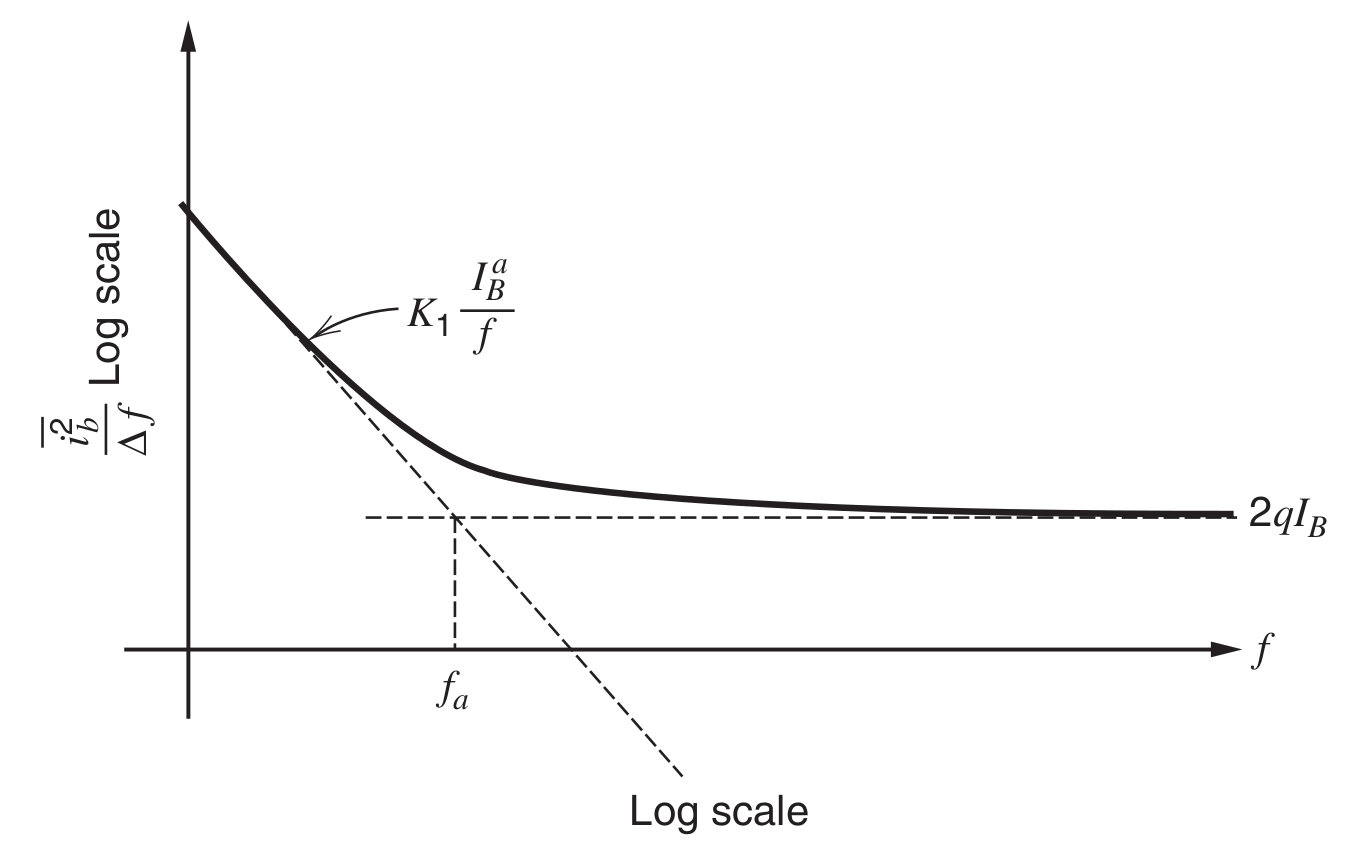
\includegraphics[width=0.6\textwidth]{figures/corner-frequency.png}
	\caption{Power spectral density of the base-current noise generator in a
	bipolar transistor. At low frequency, $1/f$ noise dominates while at higher
	frequency, shot noise dominates. $f_a$ is called the flicker noise
	\emph{corner} frequency.}
	\label{fig:corner-frequency}
\end{figure}

\subsubsection{MOS transistor}
A small-signal model equivalent circuit with noise sources for the MOS transistor
is given in figure~\ref{fig:mos-noise-model}. This model contains the following
noise sources:
\begin{enumerate}
    \item $\mean{i^2_g}$ : contains the shot noise generated by the gate leakage current
    \[ \mean{i^2_g} = 2qI_G\Delta f. \]
    At higher frequencies, another noise component due to a random component of the
    gate-to-channel voltage caused by thermal noise along the channel. This generates
    a noisi ac gate current $i_g$ with mean-squared value
    \[ \mean{i^2_g} = \frac{16}{15}kT\omega^2C^2_{gs}\Delta f. \]
    \item $\mean{i^2_d}$ : since the channel material is resistive, it exhibits thermal
    noise, which is a major source of noise in MOS transistors. Moreover, because MOS
    transistors conduct current near the surface of the silicon where surface states acts
    as traps that capture and release current carries: this generates flicker noise.
    \[
        \mean{i^2_d} = 4kT\left(\frac{2}{3}g_m\right)\Delta f + K\frac{I_D^a}{f^b}\Delta f
    \]
    where $\frac{2}{3}g_m$ models the channel resistance.
\end{enumerate}

\begin{figure}[ht]
    \centering
    \begin{circuitikz}
        \draw
        (0, 2) to[short, o-, l=$G$] (1, 2)
        (0, 0) to[short, o-] (1, 0) to[I, i=$\mean{i^2_g}$] (1,2)
        (1, 2) -- (3, 2) to[C, l_=$C_{gs}$, v^=$v_{gs}$] (3, 0) -- (1, 0)
        (3, 2) to[C, l^=$C_{gd}$] (5, 2) to[I, i=$g_mv_{gs}$] (5, 0)
        (5, 0) to[short, -, l^=$S$] (3, 0)
        (5, 2) -- (7, 2) to[R, l=$r_o$] (7, 0) -- (5, 0)
        (7, 0) -- (9, 0) to[I, i=$\mean{i^2_d}$] (9, 2) -- (7, 2)
        (9, 0) to[short, -o] (10, 0)
        (9, 2) to[short, -o, l^=$D$] (10, 2)
        ;
    \end{circuitikz}
    \caption{The MOS transistor small-signal equivalent circuit
    with noise sources.}
    \label{fig:mos-noise-model}
\end{figure}

\subsection{Circuit noise calculations}
\subsubsection{Superposition}
When two sources of voltage noises are in series, they can be grouped
in a equivalent source of voltage noise $\mean{v^2_e}$ as illustrated
in figure~\ref{fig:superposition-voltage}.

\begin{figure}
    \centering
    \begin{circuitikz}
        \draw
        (0,0) to[short, o-] (0,-0.5)
        (0,-2) to[V, v=$\mean{v_1^2}$] (0,-0.5)
        (0,-3.5) to[V, v=$\mean{v_2^2}$] (0,-2)
        (0,-3.5) to[short, -o] (0,-4)
        
        (2,-2.5) node[label=$\to$]{}
        
        (4,0) to[short, o-] (4,-0.5)
        (4,-3.5) to[V, v=$\mean{v_e^2}$] (4,-0.5)
        (4,-3.5) to[short, -o] (4,-4)
        ;
    \end{circuitikz}
    \caption{Superposition principle for noise voltage generators. A similar
    principle applies for noise current generators.}
    \label{fig:superposition-voltage}
\end{figure}
The relation between $\mean{v^2_e}$ and $\mean{v_1^2}$ and $\mean{v_2^2}$
depends on the relation between $v_1$ and $v_2$.

\begin{itemize}
    \item Non-correlated sources:
    \[ \mean{v^2_e} = \mean{v^2_1} + \mean{v^2_1} \]

    \item Fully correlated sources:
    \[ \mean{v^2_e} = \mean{(v_1+v_2)^2} \]

    \item Partially correlated sources:
    let $v_2 = v_{22} + v_{21}$ where $v_{22}$ is non-correlated with $v_1$
    and $v_{21}$ is fully correlated with $v_1$. In this case,
    \[ \mean{v^2_e} = \mean{(v_1 + v_{21})^2} + \mean{v^2_{22}}. \]
\end{itemize}

\subsubsection{Output noise}
Here are the steps involved in the computation of the total output noise
\begin{enumerate}
    \item Draw the small-signal equivalent circuit with noise sources ;
    \item Ignore the external input signal $v_i$ so that the output signal
    $v_o$ is due to noise generators only ;
    \item Apply the superposition principle and consider each noise source at
    a time. Perform the calculation as if each noise source were a sinusoid with
    rms value equal to that of the noise source being considered ;
    \item Combine every noise sources as explained in the previous section (i.e.,
    depending on their independence).
\end{enumerate}
A complete example can be found in~\cite[section~11.4.1]{gray}.

\subsubsection{Equivalent input noise and the minimum detectable signal}
The previous section showed us how to compute the output noise. The significance
of the noise performance of a circuit is, however, the limitation it places on
the smallest input signal the circuit can handle before the noise degrades the
quality of the output signal. For this reason, the noise performance is usually
expressed in terms of an equivalent input noise signal, which gives the same output
noise as the circuit under consideration.
The situation is illustrated in figure~\ref{fig:eq-input-noise}. The need for both
an equivalent input noise voltage generator and an equivalent input noise current
generator to represent the noise performance of the circuit for any source resistance
can be appreciated as follows. If $R_S = 0$, then $\mean{i^2_i}$ is shorted out, and
since the original circuit will still show output noise in general, we need an
equivalent input noise voltage $\mean{v^2_i}$ to represent this behavior. Similarly,,
if $R_S \to\infty$, then $\mean{v^2_i}$ cannot produce output noise, and since the
original circuit will still show output noise in general, we need an equivalent
input noise current $\mean{i^2_i}$ to represent this behavior.

\paragraph{Method}
In both cases, the output of both circuits (i.e. the original one and the one with
equivalent input noise generators) must be short-circuited.
\begin{enumerate}
    \item To obtain $\mean{v_i^2}$ : short-circuit the input of both circuits
    (as discussed above, this has for effect to remove the input noise current
    generator $\mean{i_i^2}$ effect) and equate $i_o$ in each case to obtain $v_i$.
    \item To obtain $\mean{i_i^2}$ : let open-circuited the input of both
    circuits (removing the input noise voltage generator $\mean{v_i^2}$ effect).
\end{enumerate}

Examples can be found in~\cite[sections~11.5.1-2]{gray}.

\begin{figure}
    \centering
    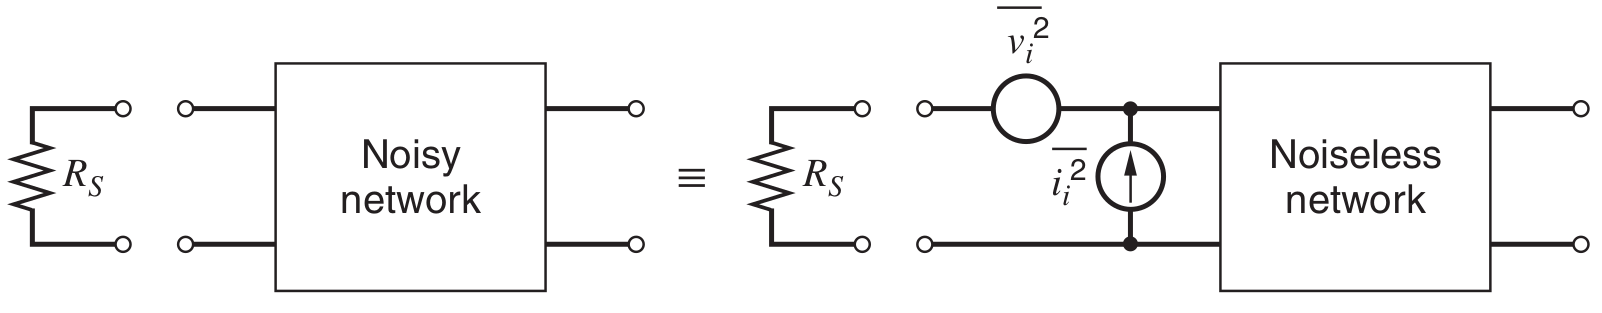
\includegraphics[width=0.75\textwidth]{figures/eq-input-noise.png}
    \caption{Representation of a noise in a two-port network equivalent input
    voltage and current generators.}
    \label{fig:eq-input-noise}
\end{figure}

\begin{mydef}[Minimum detectable signal]
    The minimum detectable signal (abbreviated MDS) can be taken as equal to
    the equivalent input noise voltage in the passband of the circuit under
    consideration.
\end{mydef}



\section{Active filters}

\section{Voltage references}

\section{DAC}

\section{ADC}

\nocite{*}
\bibliographystyle{plain}
\bibliography{biblio}

\end{document}
